\subsection{Captura 4 - Shopping Unicenter}

Esta ultima captura se realizo en el Shopping Unicenter durante treinta minutos. Durante este tiempo se capturaron $58510$ paquetes, de los cuales $2460$ fueron paquetes ARP.
En esta red se registraron $2300$ nodos. Como no es posible graficar tantos nodos de forma clara dentro de las dimensiones de una hoja A4 decidimos filtrar la mayoría.
El filtro fue motivado por la forma del digrafo de la red. En él observamos que $2294$ de los nodos sólo tenían aristas a sí mismos y los otros $6$ formaban una pequeña componente conexa.
Decidimos entonces tomar $9$ nodos que sólo estaban conectados con sigo mismos, para representar a todo ese conjunto, y a la componente conexa de $6$ nodos para realizar el digrafo de la red.
El gráfico de barras y el histograma los realizamos en función de los $6$ nodos de la componente conexa y algunos nodos \textit{solitarios}.

\begin{figure}[H]
  \centering
    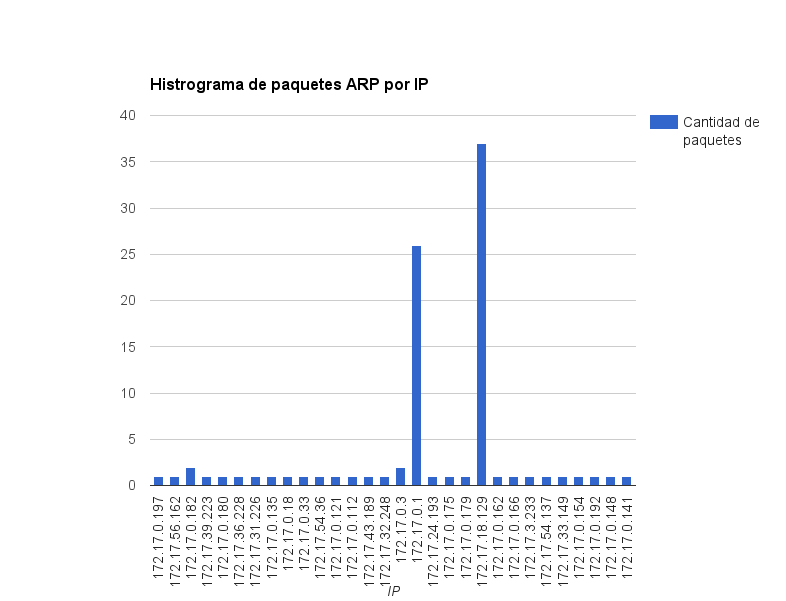
\includegraphics[width=1.1\textwidth]{imagenes/unicenter/histograma.png}
    \caption{Histograma de los símbolos de la fuente $S_{IP}$}
  \label{fig:ejemplo}
\end{figure}

Al igual que en la captura en los Laboratorios hay dos nodos que presentan una frecuencia alta, \textit{172.17.18.129} y \textit{172.17.0.1}. Notamos que esta red es la primera
que presenta nodos con IPs que comienzan con el número 172. Las IPs que pertenecen al rango \textit{172.16.0.0}-\textit{172.31.255.255} no son públicamente routeables y se reservan para el
uso de LANs privadas\footnote{Fuente: \url{https://www.arin.net/knowledge/address_filters.html}}.

\begin{figure}[H]
  \centering
    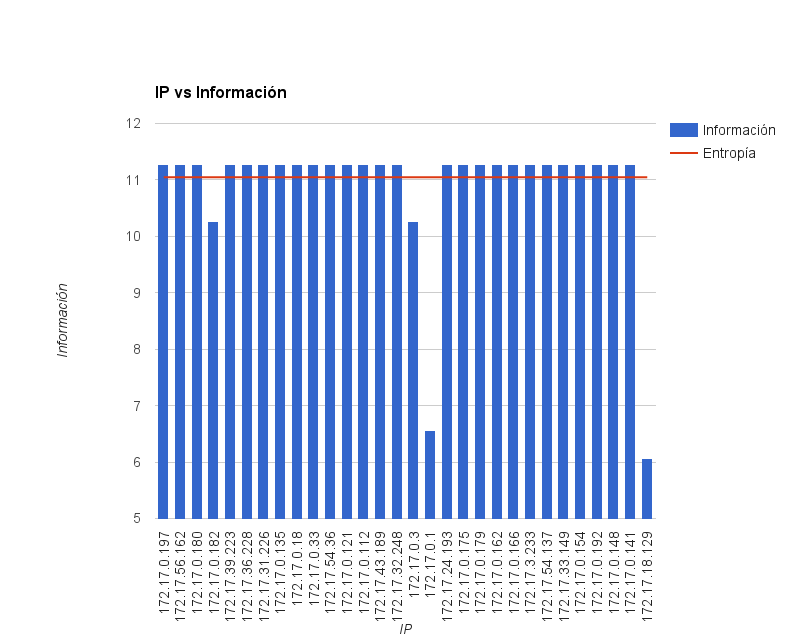
\includegraphics[width=1.1\textwidth]{imagenes/unicenter/ip_informacion.png}
    \caption{Información de los símbolos de la fuente $S_{IP}$}
  \label{fig:ejemplo}
\end{figure}

Podemos ver que muchos símbolos tienen el mismo valor de información. Esto es debido a que \textit{la gran mayoría} de los nodos de la red solo enviaron una pequeña cantidad de paquetes ARP a si mismos.

\begin{figure}[H]
  \centering
    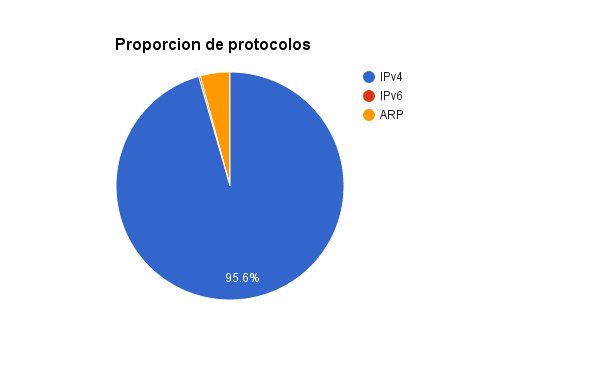
\includegraphics[width=0.7\textwidth]{imagenes/unicenter/proporcion_protocolos.png}
  \caption{Proporción de protocolos observados en el trafico de la red del shopping Unicenter}
  \label{fig:ejemplo}
\end{figure}

Nuevamente vemos que IPv4 es quien predomina en la red.
Por otra parte, el overhead impuesto por ARP es mínimo, inferior al $4\%$. Esto nos llama la atención ya que en una red pública, como fue el caso de Starbucks, esperábamos mayor necesidad del mismo.

\begin{figure}[H]
  \centering
    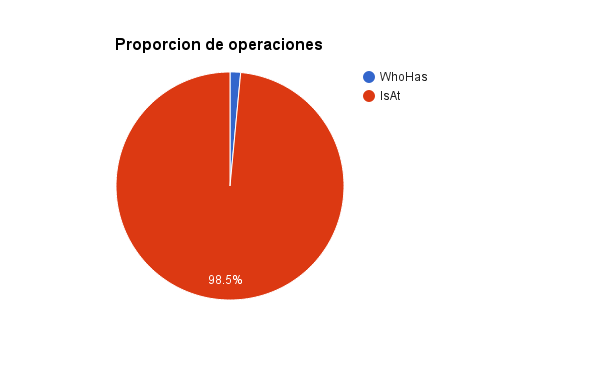
\includegraphics[width=0.9\textwidth]{imagenes/unicenter/proporcion_paquetes_arp.png}
  \caption{Proporción de paquetes who-has vs is-at en red del shopping Unicenter}
  \label{fig:ejemplo}
\end{figure}

En esta red puede verse que la proporción de paquete \textit{who-has} e \textit{is-at} es totalmente inversa a la obtenida en las tres capturas anteriores. Este comportamiento nos resulta sumamente curioso e inexplicable.

\begin{figure}[H]
  \centering
    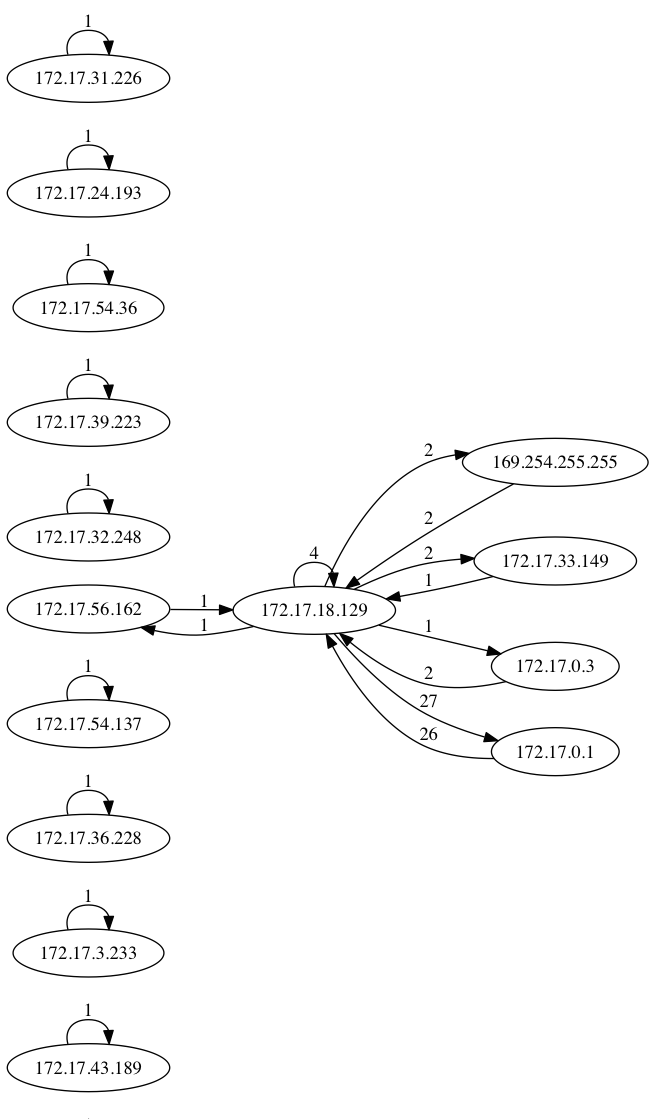
\includegraphics[width=0.48\textwidth]{imagenes/unicenter/digrafo_unicenter.png}
  \caption{Trafico de paquetes ARP entre las IP de la red del shopping Unicenter}
  \label{fig:ejemplo}
\end{figure}

No logramos explicar por qué registramos tantos nodos aislados que sólo se enviaban paquetes a sí mismos y no tenían interacción alguna con otros nodos, éste fue el caso de más del $99\%$ de los nodos.
